\documentclass[../../main.tex]{subfiles}
\begin{document}

\begin{flushright}
\footnotesize\textit{【自動文字起こし・要確認】}
\end{flushright}

% [構想メモ]
% r(P)は X, Y の2変数関数。
% → 円が A, B, C に含まれる条件
% r <= X, r <= Y, r <= 1/2(-\sqrt{3}X + \sqrt{3} - Y)
% の値域を1変数消してグラフに表し, そのうち max をとっていけば良いが...
% 1つ注意すべきは

{\bf [解]} $P(X,Y)$ とおく．$l: y = -\sqrt{3}x + \sqrt{3}$ とおく．

\begin{figure}[htb]
\centering
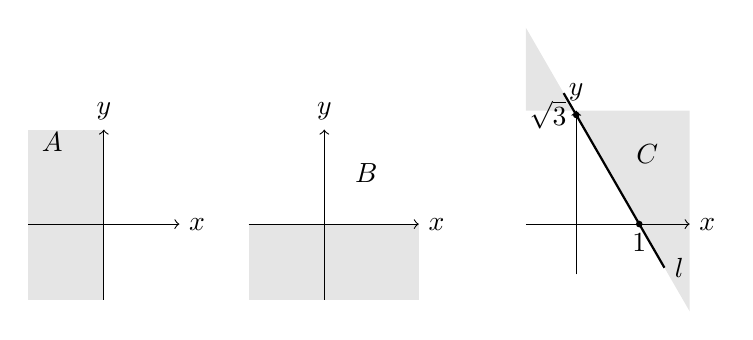
\begin{tikzpicture}[scale=0.8]
  % Region A
  \begin{scope}[shift={(0,0)}]
    \fill[gray!20] (-1.2,-1.2) rectangle (0,1.5);
    \draw[->] (-1.2,0) -- (1.2,0) node[right] {$x$};
    \draw[->] (0,-1.2) -- (0,1.5) node[above] {$y$};
    \node[above left] at (-0.5,1.0) {$A$};
  \end{scope}

  % Region B
  \begin{scope}[shift={(3.5,0)}]
    \fill[gray!20] (-1.2,-1.2) rectangle (1.5,0);
    \draw[->] (-1.2,0) -- (1.5,0) node[right] {$x$};
    \draw[->] (0,-1.2) -- (0,1.5) node[above] {$y$};
    \node[above left] at (1.0,0.5) {$B$};
  \end{scope}

  % Region C
  \begin{scope}[shift={(7.5,0)}]
    \fill[gray!20] (-0.8,{sqrt(3)*(1+0.8)}) -- (1.8,{sqrt(3)*(1-1.8)}) -- (1.8,1.8) -- (-0.8,1.8) -- cycle;
    \draw[->] (-0.8,0) -- (1.8,0) node[right] {$x$};
    \draw[->] (0,-0.8) -- (0,1.8) node[above] {$y$};
    \draw[thick] (-0.2,{sqrt(3)*(1+0.2)}) -- (1.4,{sqrt(3)*(1-1.4)}) node[right] {$l$};
    \node[above right] at (0.8,0.8) {$C$};
    \node[left] at (0,{sqrt(3)}) {$\sqrt{3}$};
    \node[below] at (1,0) {$1$};
    \fill (0,{sqrt(3)}) circle (1.5pt);
    \fill (1,0) circle (1.5pt);
  \end{scope}
\end{tikzpicture}
\caption{領域 $A,B,C$ と直線 $l$}
\end{figure}

\paragraph{(1)}

$P$ が下図斜線部をうごく時，$Y < 0 \quad (0 \le X \le 1)$ または $Y \le -\sqrt{3}X + \sqrt{3} \quad (1 < X)$ とかける．

\begin{enumerate}
  \item[$1^\circ$] 円が $A$ に含まれる時
  \begin{align}
  r \le X
  \end{align}
  \item[$2^\circ$] 円が $C$ に含まれる時
  \begin{align}
  r \le \dfrac{|\sqrt{3}X + Y - \sqrt{3}|}{\sqrt{1+3}} = \dfrac{1}{2}(-\sqrt{3}X - Y + \sqrt{3})
  \end{align}
\end{enumerate}

だから，$\alpha, \beta$ のうち小さくない方を $\max\{\alpha, \beta\}$ と表すと，
\begin{align}
r(P) = \max\Bigl\{ X, \dfrac{1}{2}(-\sqrt{3}X - Y + \sqrt{3}) \Bigr\}
\end{align}
である．$X$ を固定して，$Y$ をうごかすと $-\sqrt{3}X - Y + \sqrt{3}$ は $Y$ の単調減少関数だから，
\begin{align}
-\sqrt{3}X - Y + \sqrt{3} \begin{cases} > -\sqrt{3}X + \sqrt{3} & (0 \le X \le 1) \\ \ge 0 & (1 < X) \end{cases}
\end{align}
だから，$r(P)$ のグラフは右図のようになり，
\begin{align}
r(P) \ge -3 + 2\sqrt{3}
\end{align}

\paragraph{(2)}

$P$ の場所を以下のように場合分けする．この時，$A \cup B \cup C$ は平面全体を表すことに注意する．又，以下境界は全て含むとする．

\begin{figure}[htb]
\centering
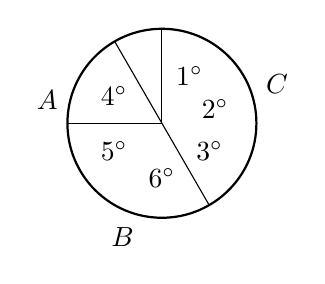
\begin{tikzpicture}[scale=1.0]
  \draw[thick] (0,0) circle (1.2cm);
  \draw (0,0) -- (0,1.2);
  \draw (0,0) -- (-1.2,0);
  \draw (0,0) -- (120:1.2cm);
  \draw (0,0) -- (-60:1.2cm);
  \node at (60:0.7cm) {$1^\circ$};
  \node at (15:0.7cm) {$2^\circ$};
  \node at (150:0.7cm) {$4^\circ$};
  \node at (210:0.7cm) {$5^\circ$};
  \node at (270:0.7cm) {$6^\circ$};
  \node at (330:0.7cm) {$3^\circ$};
  \node[left] at (-1.2,0.3) {$A$};
  \node[below] at (-0.5,-1.2) {$B$};
  \node[right] at (1.2,0.5) {$C$};
\end{tikzpicture}
\caption{領域 $A,B,C$ の重なりによる場合分け $1^\circ \sim 6^\circ$}
\end{figure}

\begin{enumerate}
  \item[$1^\circ$] $P$ が $A \cap B \cap C$ をうごく時
  \begin{align}
  0 \le Y \le -\sqrt{3}X + \sqrt{3} \quad (0 \le X \le 1)
  \end{align}
  である．
  \begin{align}
  A \text{ に含まれる} &\dots r \le X \\
  B \text{ に含まれる} &\dots r \le Y \\
  C \text{ に含まれる} &\dots r \le \dfrac{1}{2}(-\sqrt{3}X - Y + \sqrt{3})
  \end{align}
  だから，$r(P) = \max\Bigl\{ X, Y, \dfrac{1}{2}(-\sqrt{3}X - Y + \sqrt{3}) \Bigr\}$ である．まず，
  \begin{align}
  Y \ge \dfrac{1}{2}(-\sqrt{3}X - Y + \sqrt{3}) \iff Y \ge \dfrac{1}{3}(-\sqrt{3}X + \sqrt{3})
  \end{align}
  だから，
  \begin{align}
  \begin{cases}
  0 \le Y \le \dfrac{1}{3}(-\sqrt{3}X + \sqrt{3}) \text{ の時 } r(P) = \max\Bigl\{ X, \dfrac{1}{2}(-\sqrt{3}X - Y + \sqrt{3}) \Bigr\} & \dots \text{1-①} \\
  \dfrac{1}{3}(-\sqrt{3}X + \sqrt{3}) \le Y \le \sqrt{3}(-X + 1) \text{ の時 } r(P) = \max \{ X, Y \} & \dots \text{1-②}
  \end{cases}
  \end{align}
  で $X$ を固定して $Y$ をうごかすと，
  \begin{align}
  \text{1-①の時} \quad &\dfrac{1}{3}\sqrt{3}(-X+1) \le \dfrac{1}{2}(-\sqrt{3}X - Y + \sqrt{3}) \le \dfrac{\sqrt{3}}{2}(-X+1) \\
  \text{1-②の時} \quad &\dfrac{1}{3}\sqrt{3}(-X+1) \le Y \le \sqrt{3}(-X+1)
  \end{align}
  でグラフは右図で
  \begin{align}
  r(P) \ge \dfrac{-1 + \sqrt{3}}{2} \quad \dots *
  \end{align}

  \item[$2^\circ$] $P$ が $A \cap B \cap \overline{C}$ をうごく時
  
  $A$ に含まれる $\dots r \le X$，$B$ に含まれる $\dots r \le Y$ から，
  $r(P) = \max(X, Y)$ であり，又
  \begin{align}
  \begin{cases}
  \dfrac{1}{\sqrt{3}}(-\sqrt{3}X + \sqrt{3}) \le Y & (0 \le X \le 1) \\
  0 \le Y & (1 \le X)
  \end{cases}
  \end{align}
  だから，グラフは右図で
  \begin{align}
  r(P) \ge \dfrac{1}{2}(3 - \sqrt{3}) \quad \dots *
  \end{align}

  \item[$3^\circ$] $P$ が $\overline{A} \cap B \cap C$ をうごく時
  
  $B$ に含まれる $\dots r \le Y$，$C$ に含まれる $\dots r \le \dfrac{1}{2}(-\sqrt{3}X - Y + \sqrt{3})$ で，$0 \le Y \le \sqrt{3}(-X+1) \quad (X \le 0)$ である．よって，
  \begin{align}
  \begin{cases}
  0 \le Y \le \dfrac{\sqrt{3}}{3}(-X+1) \text{ の時 } r(P) = \dfrac{1}{2}(-\sqrt{3}X - Y + \sqrt{3}) \\
  \dfrac{\sqrt{3}}{3}(-X+1) \le Y \le \sqrt{3}(-X+1) \text{ の時 } r(P) = Y
  \end{cases}
  \end{align}
  左図から，
  \begin{align}
  r(P) \ge \dfrac{\sqrt{3}}{3} \quad \dots *
  \end{align}

  \item[$4^\circ$] $P$ が $A \cap \overline{B} \cap \overline{C}$ をうごく時
  
  $1 \le X$ で，$r(P) = X$ から
  \begin{align}
  r(P) \ge 1 \quad \dots *
  \end{align}

  \item[$5^\circ$] $P$ が $\overline{A} \cap \overline{B} \cap \overline{C}$ をうごく時
  
  $1 \le Y$ で，$r(P) = Y$ から
  \begin{align}
  r(P) \ge 1 \quad \dots *
  \end{align}

  \item[$6^\circ$] $P$ が $\overline{A} \cap \overline{B} \cap C$ をうごく時
  
  $X, Y \le 0$ で，$r(P) = \dfrac{1}{2}(-\sqrt{3}X - Y + \sqrt{3})$ から
  \begin{align}
  r(P) \ge \dfrac{\sqrt{3}}{2} \quad \dots *
  \end{align}
\end{enumerate}

以上 $1^\circ \sim 6^\circ$ から，
\begin{align}
\min r(P) = \dfrac{-1 + \sqrt{3}}{2}
\end{align}

\end{document}
